% Chapter Template

\chapter{Ejemplos Latex} % Main chapter title

\label{EjemplosLatex} % Change X to a consecutive number; for referencing this chapter elsewhere, use \ref{ChapterX}

\lhead{Ejemplos Latex. \emph{Ejemplos Latex}} % Change X to a consecutive number; this is for the header on each page - perhaps a shortened title

%----------------------------------------------------------------------------------------
%       SECTION 1
%----------------------------------------------------------------------------------------





\section{Codigo XML}


Para poner codigo xml dentro del documento

\begin{lstlisting}
<?xml version="1.0" encoding="utf-8"?>
<xs:schema attributeFormDefault="unqualified" elementFormDefault="qualified"
   xmlns:xs="http://www.w3.org/2001/XMLSchema">
  <xs:element name="points">
    <xs:complexType>
      <xs:sequence>
        <xs:element maxOccurs="unbounded" name="point">
          <xs:complexType>
            <xs:attribute name="x" type="xs:unsignedShort" use="required"/>
            <xs:attribute name="y" type="xs:unsignedShort" use="required"/>
          </xs:complexType>
        </xs:element>
      </xs:sequence>
    </xs:complexType>
  </xs:element>
</xs:schema>
\end{lstlisting}

Un poco mas pequeno
\begin{lstlisting}[basicstyle=\ttfamily\tiny]
<?xml version="1.0" encoding="utf-8"?>
<xs:schema attributeFormDefault="unqualified" elementFormDefault="qualified"
   xmlns:xs="http://www.w3.org/2001/XMLSchema">
  <xs:element name="points">
    <xs:complexType>
      <xs:sequence>
        <xs:element maxOccurs="unbounded" name="point">
          <xs:complexType>
            <xs:attribute name="x" type="xs:unsignedShort" use="required" />
            <xs:attribute name="y" type="xs:unsignedShort" use="required" />
          </xs:complexType>
        </xs:element>
      </xs:sequence>
    </xs:complexType>
  </xs:element>
</xs:schema>
\end{lstlisting}



\section{varias columnas}

Para poner texto en varias columnas

\begin{multicols}{2}
 Datos en dos columnas fndio fpeowu fpieuwpu piud pqeudp oquewp duqwipud
 pqwudpqwiodu pqwidu pqwidu pqwiud piqwud pqwu dpqwoud pqwod qpwodu qwpdu
 qwpd upou pqowdu wpqo po uqwpod u
\end{multicols}



\section{Figuras}

Esta figura se pone exactamente donde se define. No se deja a latex elegir
el sitio

\begin{figure}[htbp]
\centering
\[
 \begin{matrix} 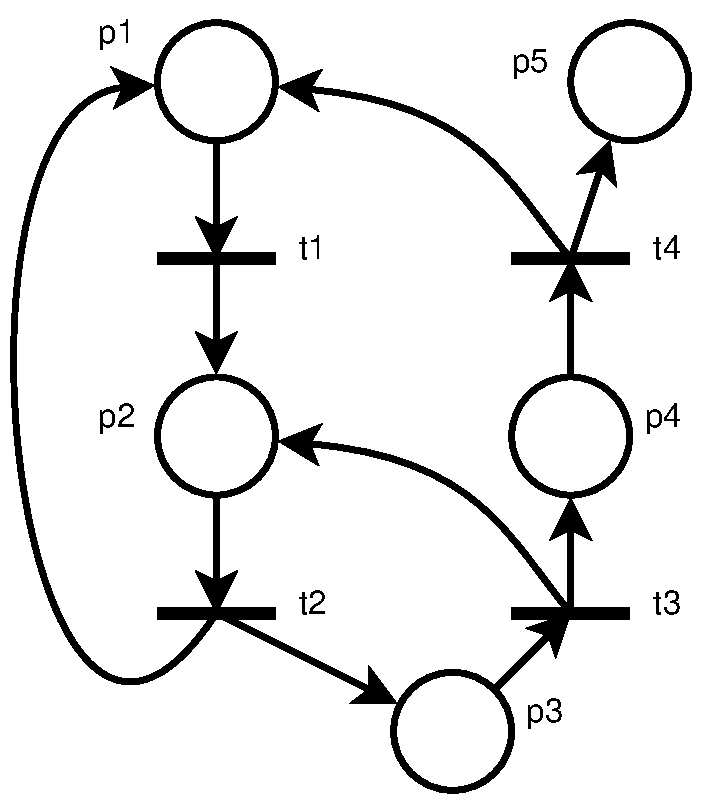
\includegraphics[width=0.3\textwidth]{Figures/EleccionSubredZonasInfluencia_1.eps}\end{matrix}
  \ \ \ \equiv \ \ \ 
 \begin{matrix}  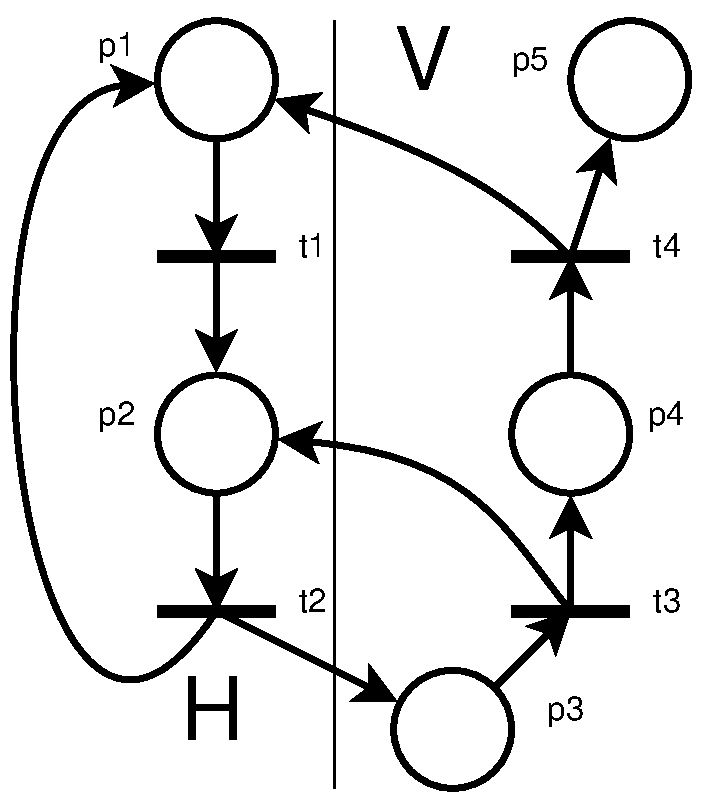
\includegraphics[width=0.3\textwidth]{Figures/EleccionSubredZonasInfluencia_2.eps}\end{matrix}
\]
\rule{35em}{0.5pt}
 \caption{figura con dos partes y que se pone exactamente donde se define}
 \label{fig:figura con dos partes 1} 
\end{figure}
 

Sin embargo esta otra la elige latex

\begin{figure}
\centering
\[
 \begin{matrix} 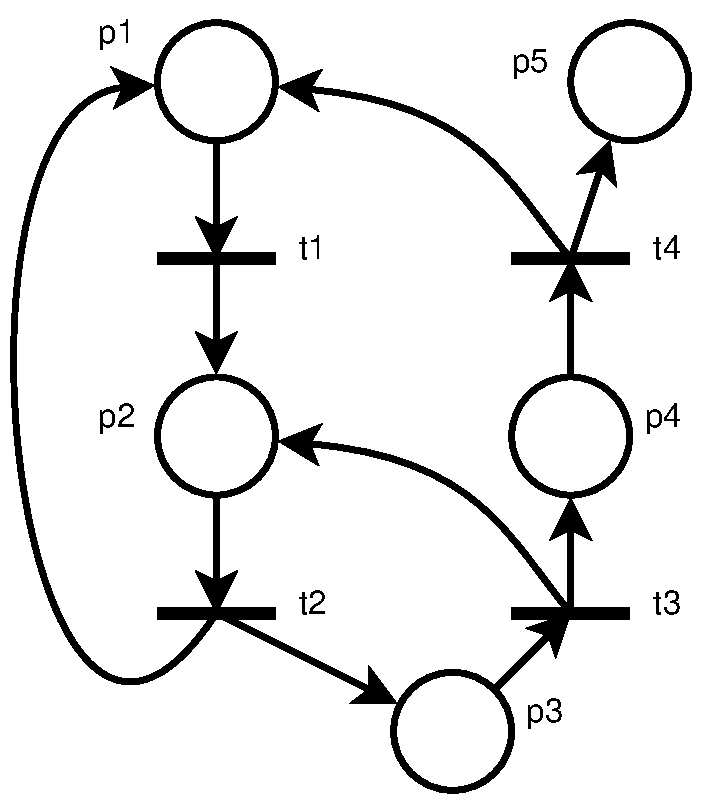
\includegraphics[width=0.3\textwidth]{Figures/EleccionSubredZonasInfluencia_1.eps}\end{matrix}
  \ \ \ \equiv \ \ \ 
 \begin{matrix}  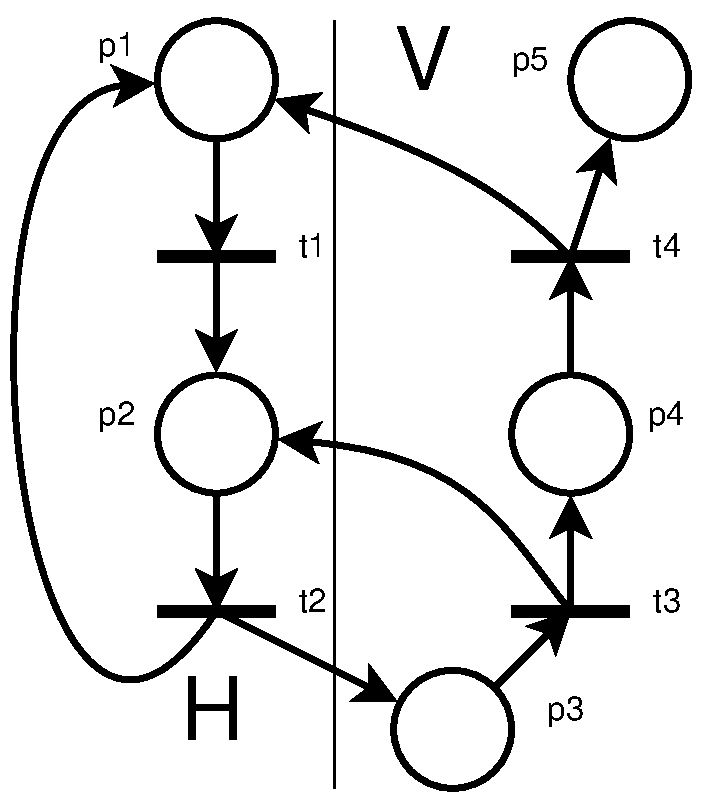
\includegraphics[width=0.3\textwidth]{Figures/EleccionSubredZonasInfluencia_2.eps}\end{matrix}
\]
\rule{35em}{0.5pt}
 \caption{figura con dos partes general}
 \label{fig:figura con dos partes 2} 
\end{figure}


